%Monthly report for the PuMA fuel meter project
%Created by Doug Keller

\documentclass[12pt,a4paper]{article}

\usepackage{fancyhdr,url,graphicx,caption,tabu,varwidth}
\usepackage[a4paper, top = 1in, bottom = 1in, left = .75in, right = .75in]{geometry}
\renewcommand{\familydefault}{\sfdefault}
\fancyfoot{}
\fancyhead{}
\pagestyle{fancy}

\fancyhead[L]{
\includegraphics[height = 32pt]{../Logos/acep.pdf}}
\fancyhead[R]{\includegraphics[height = 24pt]{../Logos/uaf_blue_hor.pdf}}
\fancyfoot[C]{Flip page for tips to help you save on fuel!}
\renewcommand{\headrulewidth}{0pt}

\setlength{\parindent}{0pt}
\setlength{\fboxrule}{.8pt}
\usepackage[font = footnotesize, textfont=it, labelfont= bf]{caption}

\newcommand{\totalusage}{2.845}
\newcommand{\fuelperday}{0.092}
\newcommand{\fuelprice}{3}
\newcommand{\totalcost}{8.53}
\newcommand{\fuelcostperday}{0.28}
\newcommand{\neighborusage}{3.287}
\newcommand{\percentusage}{13.45}
\newcommand{\moreless}{less}
\newcommand{\reportmonth}{May}
\newcommand{\reportyear}{2019}
\newcommand{\progress}{65.63}
\newcommand{\progressmoreless}{less}


\begin{document}

\begin{center}
\textbf{\Huge{\\{\reportmonth} {\reportyear} Fuel Usage Report}}
\end{center}

\begin{center}
\fbox{
\begin{varwidth}{.8\textwidth}
In {\reportmonth} you consumed {\percentusage}\% {\moreless} than your neighbors.
\end{varwidth}
}
\end{center}

\vspace{12pt}

\begin{tabu}[c]{llX[m,c]}

\begin{minipage}{4in}
\includegraphics[height = 2.375in]{monthly_fuel_usage.png}
\end{minipage}

 && 

\begin{minipage}{\linewidth}
\underline{{\reportmonth} {\reportyear} Fuel Usage:}\\

Total Usage: {\totalusage} gal\\

Price of Fuel: \${\fuelprice}/gal\\

Total Cost: \${\totalcost}\\
\end{minipage}


\end{tabu}

\rule{\textwidth}{1pt}
\newline

\begin{tabu}{X[m,c]X[m,c]}

\begin{minipage}{\linewidth}
\underline{In {\reportmonth:}}\\

Your average fuel consumption was {\fuelperday} gallons per day.\\

Your average fuel cost was \${\fuelcostperday} per day\\
\end{minipage}

&

\begin{minipage}{\linewidth}
\includegraphics[height = 3in]{monthly_polar_plot.png}
\end{minipage}


\end{tabu}

\rule{\textwidth}{1pt}
\newline

\underline{Track Your Progress:}\\

You consumed {\progress}\% {\progressmoreless} this month than last month.\\
\begin{center}
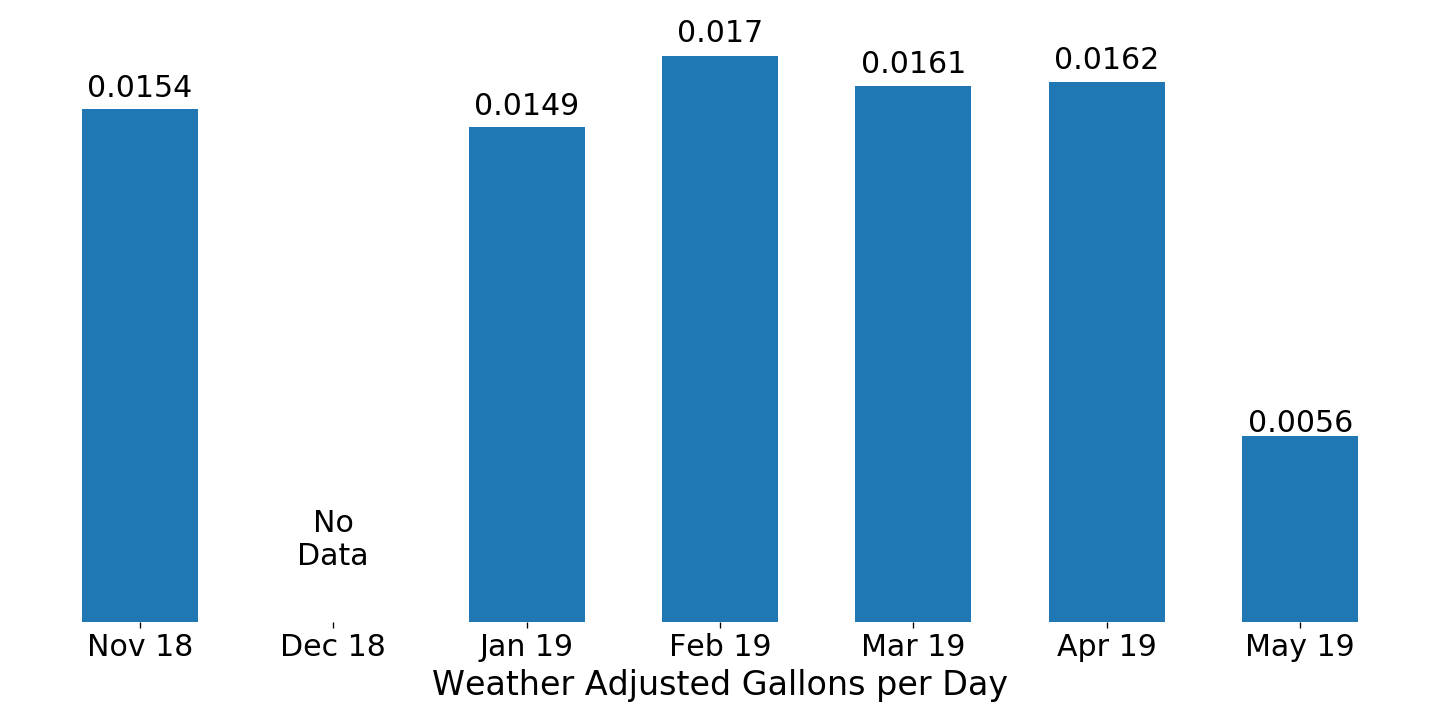
\includegraphics[height= 1.875in]{monthly_track_your_progress.png}
\end{center}

\newpage
\renewcommand{\headsep}{14pt}
\fancyfoot{}
\begin{center}
\textbf{\Huge{Tips on Saving Fuel}}
\end{center}

\vspace{12pt}
\begin{itemize}
\item Tips go here
\end{itemize}

\end{document}